\chapter{The Network Structure of Collaborative Communities}
\label{collaborative_communities}

The organization of knowledge production and diffusion has been a challenging problem for economists, sociologists and organization theorists. The increasing importance of knowledge-intensive sectors of the economy, and the inadequacies of markets and hierarchy as coordinating principles for knowledge production and diffusion, has prompted some scholars to suggest that these activities might be better organized through an alternative organizing principle: community \citep{adler:2001}. It is suggested that a new form of community, qualitatively different from the traditional \emph{Gemeinschaft} and the modern \emph{Gesellschaft} \citep{tonnies:1974}, has emerged.  Examples of collaborative communities are large scientific projects, novel forms of professional work organization \citep*{adler:2008}, open source software communities, and knowledge-intensive production processes in corporations \citep{adler:2006}.

These collaborative communities are characterized by conscious cooperation, high interdependence, trust, shared values and a value-rational basis for legitimate authority \citep{adler:2006,adler:2008}. While all these dimensions matter for a proper characterization of collaborative communities, it is clear that trust plays a more critical role as the key social mechanism of this form. But how does trust develop in these loosely coupled social forms? \citet{adler:2006} suggest that dense local interactions facilitate the emergence of trust, and common values facilitate the development of collective identity.  Scarce attention is given to the structural features of cooperation in these communities. Given the sizable literature on the social structure that facilitate (or inhibit) the emergence of trust in society \citep{granovetter:1985,coleman:1988,moody:2003}, I believe that an important question to further our understanding of collaborative communities is to explore the network structure that lead to their emergence and effectiveness in the production and diffusion of knowledge.

In this chapter therefore I suggest that a unique social network structure undergirds collaborative communities, and facilitate the development of trust and increase their robustness to turnover. Building on the literature on small world and cohesive groups, I identify the key structural feature of these networks which I call cohesive small worlds.

\section{Collaborative communities}

The concept of collaborative communities was introduced to make sense of novel organizational forms which were defying the traditional dichotomy between hierarchy and market \citep{coase:1937,williamson:1975}. \citet{ouchi:1980} was one of the first social theorist to include community/trust in the principles of social organization; he refereed to these principles as clan, but he conceptualized the relation between market, hierarchy and community as a three-way trade-off. Likewise \citet{powell:1990} introduced networks as an alternative principle to hierarchy and markets. Instead, \citet{adler:2001} considers these three principles ---Hierarchy, Market and Community--- as ideal-types which concrete organizations mix in hybrid forms.  Each one of these principles is based on a coordination mechanism. Authority is the main mechanism used in hierarchy to coordinate horizontal and vertical division of labour. Price is the mechanism through which market coordinates competing and anonymous suppliers and buyers. And trust, generated by shared values and norms, is the main mechanism of community principle \citep{adler:2001}.

This three-dimensional space allows a fine gained classification of organizations and institutions, considering the effects of the mixture of different organization principles. \citet{adler:2006} argue that, on the one hand, neither marker nor hierarchy can actually function without at least some underpinning of community and, on the other hand, that the form of community differs depending on its relation to the other two principles of social organization: ``When the dominant principle is hierarchy, community takes the form of \emph{Gemeinschaft}. When the dominant principle shifts to market, community mutates from \emph{Gemeinschaft} into \emph{Gesellschaft}. We postulate that when community itself becomes the dominant organizing principle, it will take a form quite different from either \emph{Gemeinschaft} or \emph{Gesellschaft}'' \citep[16]{adler:2006}.

This new form of community can be called collaborative community and it is based on contribution-based trust as its primary social mechanism: ``The basis of trust is the degree to which members of the community believe that others have contributions to make towards this shared [end]'' \citep[21]{adler:2006}. This form of community seems especially well suited to deal with the challenges of knowledge-based production processes because, hierarchy and market have proved ineffective, at best, at managing knowledge. On the hierarchy side, knowledge is treated as scarce resource and therefore centralized at the higher levels of the organization where key decisions are taken; this rigid scheme prevents the necessary flexibility to deal with unanticipated problems ---very common in non-routine tasks--- and to foster innovation and generation of new knowledge \citep[216]{adler:2001}. 

On the market side, the price mechanism fails to optimize the production and allocation of knowledge \citep{arrow:1962,stiglitz:1996}. The fact that knowledge is a public good that grow rather than diminish with use poses serious problems to the effectiveness of price mechanism. There is a trade-off between production and allocation: ``On one hand, production of knowledge would be optimized by establishing strong intellectual property rights that create incentives to create knowledge. On the other hand, not only are such rights difficult to enforce, but more fundamentally, they block socially optimal allocation. Allocation of knowledge would be optimized by allowing free access because the marginal cost of supplying another costumer with the same knowledge is close to zero'' \citep[217]{adler:2001}.

In conclusion: ``neither markets nor hierarchies [...] nor any intermediate forms [...] can simultaneously optimize incentives to produce knowledge and to disseminate it'' \citep[29]{adler:2006}. But community can effectively deal with knowledge production and distribution by ``reduc[ing] both transaction costs --replacing contracts with handshakes--- and agency risks ---replacing the fear of shirking and misrepresentation with mutual confidence. Community can thus greatly mitigate coordination difficulties created by knowledge's public good character'' \citep[30]{adler:2006}. The community principle of coordination allows to combine different people with different sets of knowledge and expertise in order to solve complex problems while in the process they benefit each other and their common goal.

This solution to the organization of knowledge intensive activity has helped us understand puzzling empirical cases, but few theoretical puzzle need to be addressed. Given the central role that trust play in collaborative communities, it seems essential to explore the conditions in which trust can thrive. Adler and Heckscher (2006) suggest that individuals in collaborative communities will develop higher trust because given the high interdependence of their work, they need to collaborate to achieve their common goal.  Furthermore they suggest a common value orientation facilitate the development of common identities. This approach, while based on decades of literature on trust and traditional communities, is problematic for two reasons. First of all, it is not clear how trust and value congruence emerge. Both these characteristics are neither easy to find, nor to maintain, and it is theoretically critical to ask ourselves if there are factors that can explain both. Moreover, it is not clear how trust and shared values can be maintained in large heterogeneous geographically distributed communities where membership exhibits high turnover (a common feature of many concrete collaborative communities). 

I argue that the current characterization of collaborative community can be fruitfully enriched with the growing literature on social networks, in order to identify the structural conditions that enable trust and value congruence. A structural approach to collaborative communities is not inconsistent with what has been done so far, but will help (1) refine the current characterization of communities in social network terms, (2) provide a methodology to unobtrusively identify collaborative communities in the wild, and (3) a contribution to the existing tool-kit to design collaborative communities. I explore existing models of network of knowledge production, compare them, and suggest that there is a consistent set of topological properties that characterize collaborative communities.

\section{A network approach to collaborative communities}

A network approach to collaborative communities should start from the basic building block of collaborative activity: team work. There is evidence of a trend towards more cooperative activity, often associated with the increasing complexity and interdependence of knowledge production and creative activity more generally \citep*{guimera:2005,uzzi:2005,uzzi:2007a,jones:2008}. Based on works in science, engineering, social sciences, arts, humanities and patents, \citet{uzzi:2007a} show that until the 1950s solo-authored academic articles and inventions were more likely to receive a large number of citations than articles and inventions developed by teams.  This is not true anymore, and the trend towards collective research and teamwork is illustrated by the fact that in the last decade the top cited papers in all the disciplines studied were mostly created by teams.

The study of science as collaborative creative work, and scientific communities as collaborative communities has contributed to our understanding of the properties of the networks created by these collaborations. For instance, \citet{guimera:2005} suggest that three simple mechanisms of team assembly (number of team members, probability of team members being and incumbent, and propensity to repeat collaborations) determine the topological properties of the network structure that emerge and are correlated with the performance of the teams. They study the evolution of cooperation networks in Social Psychology, Economics, Ecology and Astronomy, and show how the network evolve from a structure characterized by isolated clusters of scientists towards one in which a large portion of them are connected (in networks terms, they all belonged to the same component: all nodes that can be connected to each other by at least one path). In all cases more than half the scientists belonged to the largest connected component of the network. The relative size of the giant component was also associated with performance (publishing in journals with high impact factor) in social psychology and ecology (but not in economics and astronomy). \citet{guimera:2005}  argue that a large connected component in a field would be an evidence of the existence of an invisible college \citep{solla:1986,merton:1979}: a network of social and professional relations linking scientists across universities, which forms a repository of resources and knowledge developed in the past collaborations of the members of the filed.  The emergence of a giant component, therefore, seems like a necessary, but clearly not sufficient feature of the network of a collaborative community.

\subsection{Networks of knowledge production: small world model}

One of the key properties of the network structure of a collaborative community should be facilitating an efficient flow of information and ideas among collaborators. The class of network models that most likely fit these requirements is the small-world model \citep{watts:1998}. Small World networks are characterized by a high level of local density of social ties and short average distances among nodes in the network. More formally,\citet{watts:1998} postulated than 2 measures can be used in order to quantify small world model: average path length ($L$) and clustering coefficient ($CC$). $L$ measures the average number of intermediaries between any two nodes of the network, which theoretically means that it is a measurement of how close resources, people and knowledge are in a concrete network. $CC$ is the mean probability that two nodes that are neighbors of the same other node will themselves be neighbors. This measure has been used as proxy for cohesion or closure of networks. The smallworldiness of a network is usually measured with the small world index $Q$ (see appendix \ref{sw-affnets} for a formal definition).

Since the publication of \citeauthor{watts:1998}'s seminal paper, an important stream of empirical studies have analyzed a wide variety of networks, spanning multiple levels of analysis, with the theoretical apparatus of the small world model. For instance, \citet{uzzi:2005} analyzed the network of artists who made Broadway musicals from 1945 to 1989. They found a non-linear association between smallworldiness and the financial and artistic performance of the musicals they produced: at low levels of $Q$ the network consists of many unconnected teams, which inhibits the circulation of new ideas and hinders creativity; as $Q$ increase there are more links among teams and those links are more local cohesive which foster creativity and exchange of ideas. But if $Q$ continues to rise beyond a threshold: ``the network increases in connectivity and cohesion to a point at which connectivity homogenizes the pool of creative material while cohesive ties promote common information exchanges, limiting the diversity of the pool of creative material and trapping artists in echo chambers of like minded collaborators'' \citep[87]{uzzi:2007}.

Studies conducted on other types of networks have not consistently replicated these findings \citep*[for a recent review see][]{uzzi:2007}. The inconsistency of the relation between small world structure and performance could be explained by the wide differences in the activities actors were engaged in, by the different measures of performance used, or by the different time frames of the analysis and to differences in the measurement of performance. In addition to these explanations, I would like to stress the fact that the small world model is based on a purely local measure of cohesion ($CC$). Therefore a high clustering coefficient only means that local teams are highly cohesive, but these teams might not be connected by anything more than a few random connections, and therefore we cannot say anything about the global connectivity of the network. As I will show in the next section, the global connectivity, and the presence of multiple redundant paths among actors, might play a role in explaining the differences in performance between small world structures in different settings. A network can have high global cohesion and connectivity without too much local cohesion, which is what Uzzi argues ``traps artists in echo chambers of like minded collaborators''.

Another interesting empirical result of studies of scientific cooperation networks, points to the role of specific actors in keeping the network together. \citet*{goyal:2006} show that the global patterns of cooperation among economists from 1970 to 1999 can be modeled as a small world. They also found that a core of interlinked star authors spanned the network shortening otherwise long path lengths. If those brokers were removed from the network, the average path length would rise sharply and the size of the giant connected component will shrink significantly. In the field of sociology \citet{moody:2004} shows that the global patterns of cooperation among authors does not follow a small world model. Furthermore he showed that the cohesion between sub-fields in sociology does not depend on a core of brokers, and the network did not fragment until all scholars with 10 collaborators were removed from the network.

In addition to facilitating the diffusion of ideas and the combination of diverse skills and pieces of knowledge, teams can also generate common social norms and trust ---another essential feature of collaborative communities.  To explain how trust can operate beyond the confine of each team it is necessary to explore its structural antecedents.

\subsection{Trust and social solidarity in networks: the structural cohesion model}
\label{scm}

Cohesion and social solidarity are central features for collaborative communities, and distinguish them from both ideal-typical hierarchies and markets. These concepts have a long and illustrious history in sociology \citep{durkheim:2008} but their precise characterization has been elusive. Much more attention has been focused on its ideational component, which is based on the members' identification with a collectivity, than on its relational component \citep{doreian:1998}, that is the structure of social relations among members of the group that facilitate the emergence of cohesion. Indeed, even the collaborative community literature focus almost solely on the ideational community, stressing the importance of collective identification.

As discussed in chapter \ref{structural_cohesion}, \citet{white:2001} and \citet{moody:2003} developed a robust operationalization of the relational dimension of social solidarity based on the graph-theoretic property of connectivity \citep{harary:1969}. They propose two equivalent definitions of structural cohesion: ``a group's structural cohesion is equal to the minimum number of actors who, if removed from the group, would disconnect the group'' and ``a group's structural cohesion is equal to the minimum number of independent paths linking each pair of actors in the group'' \citep[109]{moody:2003}. These two definitions are equivalent because of Menger's theorem\footnote{A cutset is a set of nodes that, if removed, would break the component into two or more pieces. A graph is $k$-connected ---has node connectivity $k$--- and it is called a $k$-component if it has no cutset of fewer than $k$ nodes. Menger's theorem states that a $k$-connected graph also has at least $k$ node-independent paths connecting every pair of nodes.}.

The starting point of the social cohesion in a group is a state where every actor can reach every other actor through at least one relational path. The formalization of this state in a concrete group is the size of the largest connected component. The emergence of a giant component, therefore, does not just provide the opportunity to access the invisible college \citep{guimera:2005}, but is also a minimal condition for the development of cohesion. \citet{moody:2003} argue that the removal of a few key nodes can affect the flow of knowledge, information and resources in the network. In network terms, a graph is $k$-connected and is called a $k$-component if you need to remove at least $k$ nodes to break it into more components. A 2-component, or bicomponent is a component that requires at least 2 nodes to be removed to break down connectivity.  Therefore \citet{moody:2003} convincingly argue that a biconnected component provides a baseline threshold for strong structural cohesion.

The cohesive structure of a network can be conceptualized as increasingly cohesive groups ---called cohesive blocks--- nested inside each other. As an example we can think of a group with an highly cohesive core surrounded by a less cohesive periphery \citep{borgatti:2000}. A common structural pattern in large networks is an hierarchical nesting of increasingly cohesive groups at low connectivity levels and non-overlapping highly cohesive groups at higher connectivity levels \citep[112]{moody:2003}. Those highly cohesive groups play a key role in the diffusion of the consequences of social interactions among actors in networks \citep[355-356]{white:2001}. It is usually assumed that the transmission through the network of knowledge, influence and resources generated by social interactions is limited to people 2 or 3 steps away from the initiator of such interactions. In graph theoretic terms, this means that social interactions have a high rate of decay. However, strongly cohesive blocks allow repetition of information and reinforcement of influence because they are characterized by multiple independent pathways that compensate the decay effects of the transmission of knowledge, influence and resources.

This key feature of cohesive groups provides a plausible social mechanism for the emergence and development of trust in collaborative communities. Actors in strongly cohesive groups are able to compare independent perspectives on each other through a variety of paths that flow through distinct sets of intermediaries, which provides multiple independent sources of information about other's characteristics or identity \citep[320]{white:2001}. Thus, the perception of an individual embedded in such structures of the other members of the group to whom he is not directly linked is filtered by a the perception of a variety of others whom he trusts because is directly linked to them. This mediated perception of the group generates trust at a global scale.

\subsection{Collaborative community networks: Cohesive Small Worlds}

The two models of network topology discussed above provide a solid theoretical starting point in order to analyze the characteristic network structure of collaborative communities, which, I argue, is a key element to understand trust generation and value congruence between highly heterogeneous and interdependent producers in knowledge-based production processes. Table \ref{t:models} summarizes the key dimensions along which I are comparing small world and structural cohesion, and the features I argue are critical for collaborative communities.

\begin{table}[h]
\begin{tabular}{|p{2.5cm}|p{4.5cm}|p{4.5cm}|p{4cm}|}
\hline
&Structural cohesion model&Small world model& Cohesive small world\\
\hline
Cohesion&Global cohesion: focus on cohesive groups formed by nodes linked by node-independent paths&Local Cohesion: Focus on cohesive clusters linked by few edges&Both global and local cohesion\\
\hline
Role of stars&Connectedness and cohesion are not dependent on stars&Connectedness might be highly dependent on stars&Not dependent on stars\\
\hline
Robustness&Resiliency in front of random and targeted removal of nodes&Resiliency on random removal but not necessary on targeted removal of nodes with high degree&Resiliency in front of random and targeted removal of nodes\\
\hline
Trust&Global trust among all nodes of strong cohesive groups&Local trust only among cohesive local neighborhoods& Both local and global trust\\
\hline
Source of trust&Node-independent paths between nodes&Direct links within dense local clusters& Both\\
\hline
Average path length ($L$)&Implicit: strong cohesive groups must have relative low $L$&Explicit inclusion of $L$ in the model&Explicit inclusion of $L$ in the model\\
\hline
Diffusion of social interaction&Cohesive groups as amplifiers of signals in networks&No clear mechanism; it is assumed that low $L$ is enough&Cohesive groups as amplifiers\\
\hline
\end{tabular}
\caption{Comparison of network models for collaborative communities.}
\label{t:models}
\end{table}

I want to highlight that the structural cohesion model and the small world model are not mutually exclusive. A strongly cohesive network could have an average path length comparable with its random counterpart while its clustering coefficient is significantly higher. Therefore, there are networks that fit in the intersection between the two models. In order to illustrate this fact, figure \ref{fig:models} depicts examples ---with toy graphs of 25 nodes--- of a network that is structural cohesive but not small world (figure \ref{fig:sc_grid}), a network that is small world but not structurally cohesive (figure \ref{fig:sw}) and a network that is both structurally cohesive and small world (figure \ref{fig:csw}). On the lower row of figure \ref{fig:models} there are plots of the robustness of each model in front of the deletion of nodes. Those plots depict the size of the giant component divided by the total number of nodes minus the nodes removed in the preceding steps in log scale. Red dots represent targeted removal of nodes, that is, removing nodes starting with nodes of high degree. Blue marks represent random removal of nodes, in each step I chose a node at random and remove it, error bars represent the standard deviation over 100 runs of random removal of nodes.

The example of a pure structurally cohesive network (figure \ref{fig:sc_grid}) consists in a 2 dimension grid where all nodes of the network form a giant bicomponent but its average path length is significantly higher than a random network with the same number of nodes and edges, and its clustering coefficient is 0 because there are no triangles. Therefore, this network is not a small world. This kind of network is very robust in front of targeted removal of nodes because high degree nodes are in the middle of the grid; after removing all nodes with degree 4 we still have a cycle formed by the outer edges of the original grid.

The example of a pure small world network (figure \ref{fig:sw}) is inspired in the caveman network proposed by \cite{watts:1999}. It consists in a fully connected core with 20\% of the nodes; where each node in this core is connected to a node of a fully connected subgraph of 4 nodes. Thus, the clustering coefficient of this example is significantly higher than its random counterpart but its average path length is almost the same. But, in terms of structural cohesion, the giant bicomponent is formed only by the 20\% of the nodes in the core. It should be noticed that despite the fact that this kind of network has more edges than the pure structural cohesive example, its robustness in front of targeted removal of nodes is much lower. As we can see in the robustness plot depicted in figure \ref{fig:r_sw}, if we start removing nodes with high degree, the relative size of the giant component shrinks quickly because high degree nodes are in the core of the network, and every node deleted in the core means that the fully connected subgraph of four nodes linked to it will be outside of the giant connected component. Thus, in this example, connectedness is highly dependent on stars (ie high degree nodes).

The example of a cohesive small world network (figure \ref{fig:csw}) is generated algorithmically. I start with a seed formed by a cycle network containing all the nodes in order to make sure that, in the final network, all the nodes will be in a giant bicomponent. Then I randomly link pairs of nodes until we reach the number of edges contained in a 2 dimension grid with the same number of nodes\footnote{I have chosen to limit the number of edges of the cohesive small world model to the number of edges contained in a 2 dimension grid with the same number of nodes in order to highlight that the density is not the main determinant of the robustness of a network: it is its structure. Thus, a 2 dimension grid is more robust than the cohesive small world model with the same number of edges, and the cohesive small world model is more robust than the pure small world example despite the fact that the latter has more edges}. Then I compute the small world index ($Q$) of the resultant network ---see appendix \ref{sw-affnets} for a formal definition--- and if it is lower than an arbitrary threshold I start again from the beginning until the resultant network has a small world index greater than this arbitrary threshold. For the example in figure \ref{fig:csw}, I have chosen a threshold of 1.5, but any network can be characterized as a small world if $Q > 1$.

Thus, the cohesive small world example has all its nodes in a giant bicomponent ---like the pure structural cohesive example--- but it also has almost the same average path length than its random counterpart and a clustering coefficient significantly higher ---like the pure small world example---. Figure \ref{fig:r_csw} depicts its robustness in front of targeted removal of nodes. As we can see, it is in between of the other two examples. We need to remove an important percentage of the nodes with high degree in order to shrink the size of the giant component significantly. Despite the fact that the cohesive small world example has less edges than the pure small world example, its connectedness is much less dependent on stars. Moreover, we need to remove more than 10\% of all nodes in order to be able to distinguish the effects of random and targeted removal of nodes in the relative size of the giant component. While in the pure small world example, the effects of targeted and random removal are quite different from the beginning of the removal process.

Therefore, I can conclude that the two models are not mutually exclusive. The family of networks that fit in the intersection of both models ---what I call cohesive small worlds--- exhibit consistent topological patterns. These patterns, I argue, provide the scaffolding for the emergence of collaborative communities. On the one hand, the generation of trust and congruent values among heterogeneous individuals are fostered by structurally cohesive groups in the network that play a key role in amplifying the effects of social interactions trough relatively long paths. On the other hand, the existence of highly connected local clusters allows successful cooperation among heterogeneous individuals with common interests.

\begin{landscape}
\begin{figure}[p]
\centering
\subfloat[Pure structural cohesion]{
\label{fig:sc_grid}
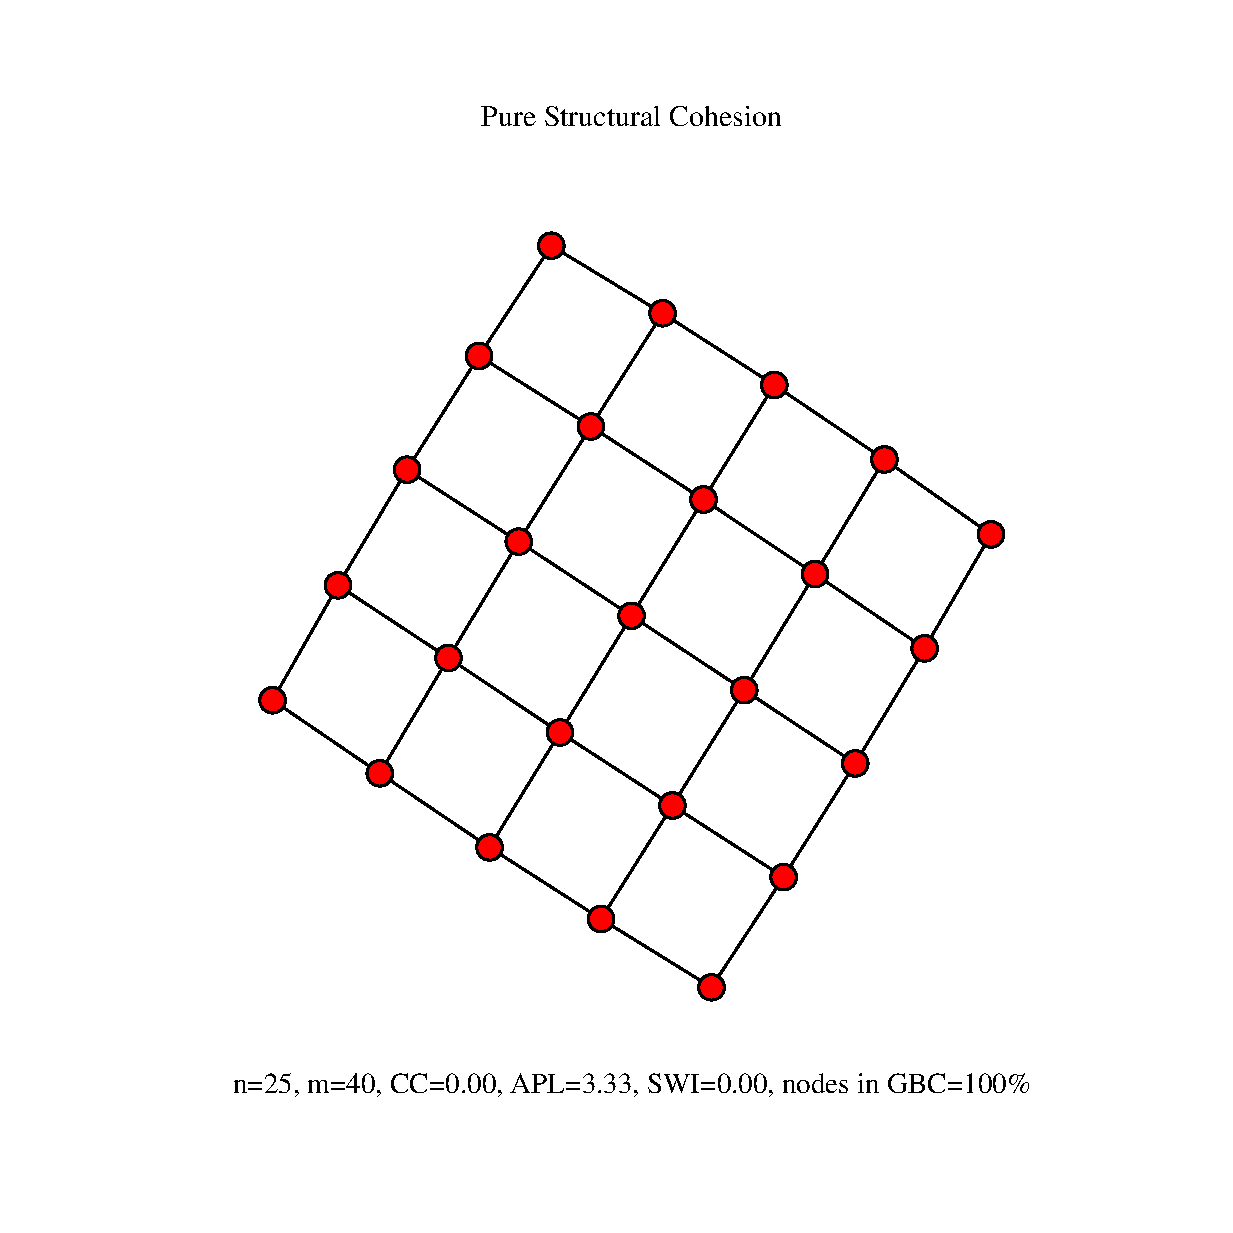
\includegraphics[scale=0.33]{figures/model_structural_cohesion_25}
}
\hspace{.05in}
\subfloat[Cohesive small world]{
\label{fig:csw}
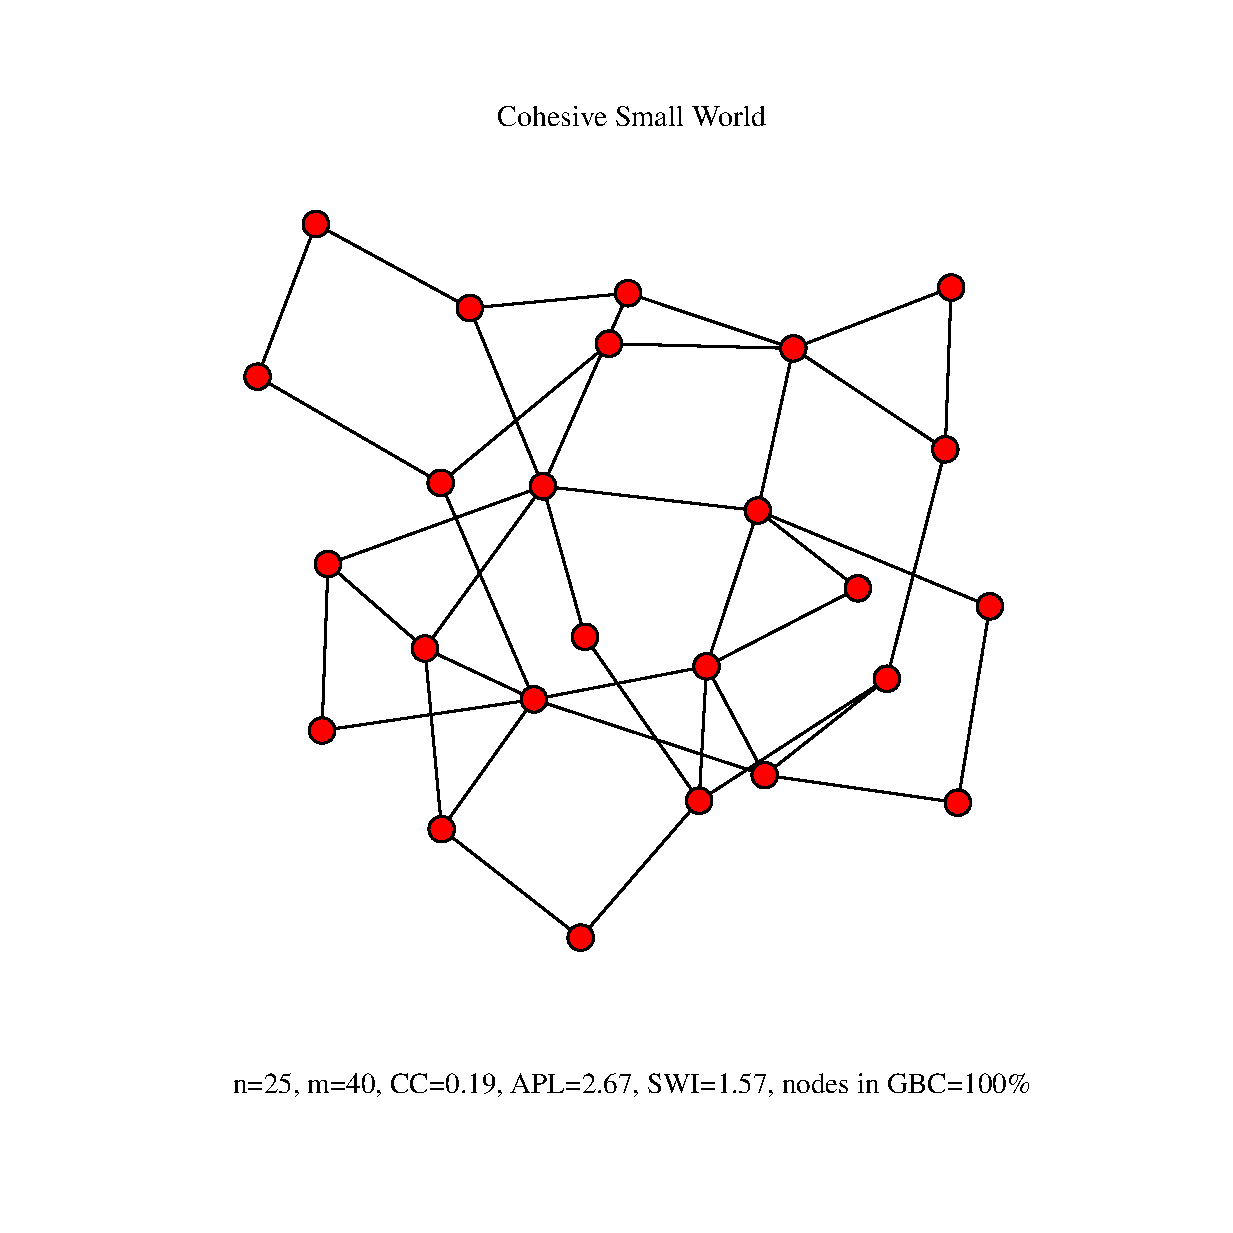
\includegraphics[scale=0.33]{figures/model_cohesive_small_world_25}
}
\hspace{.05in}
\subfloat[Pure small world]{
\label{fig:sw}
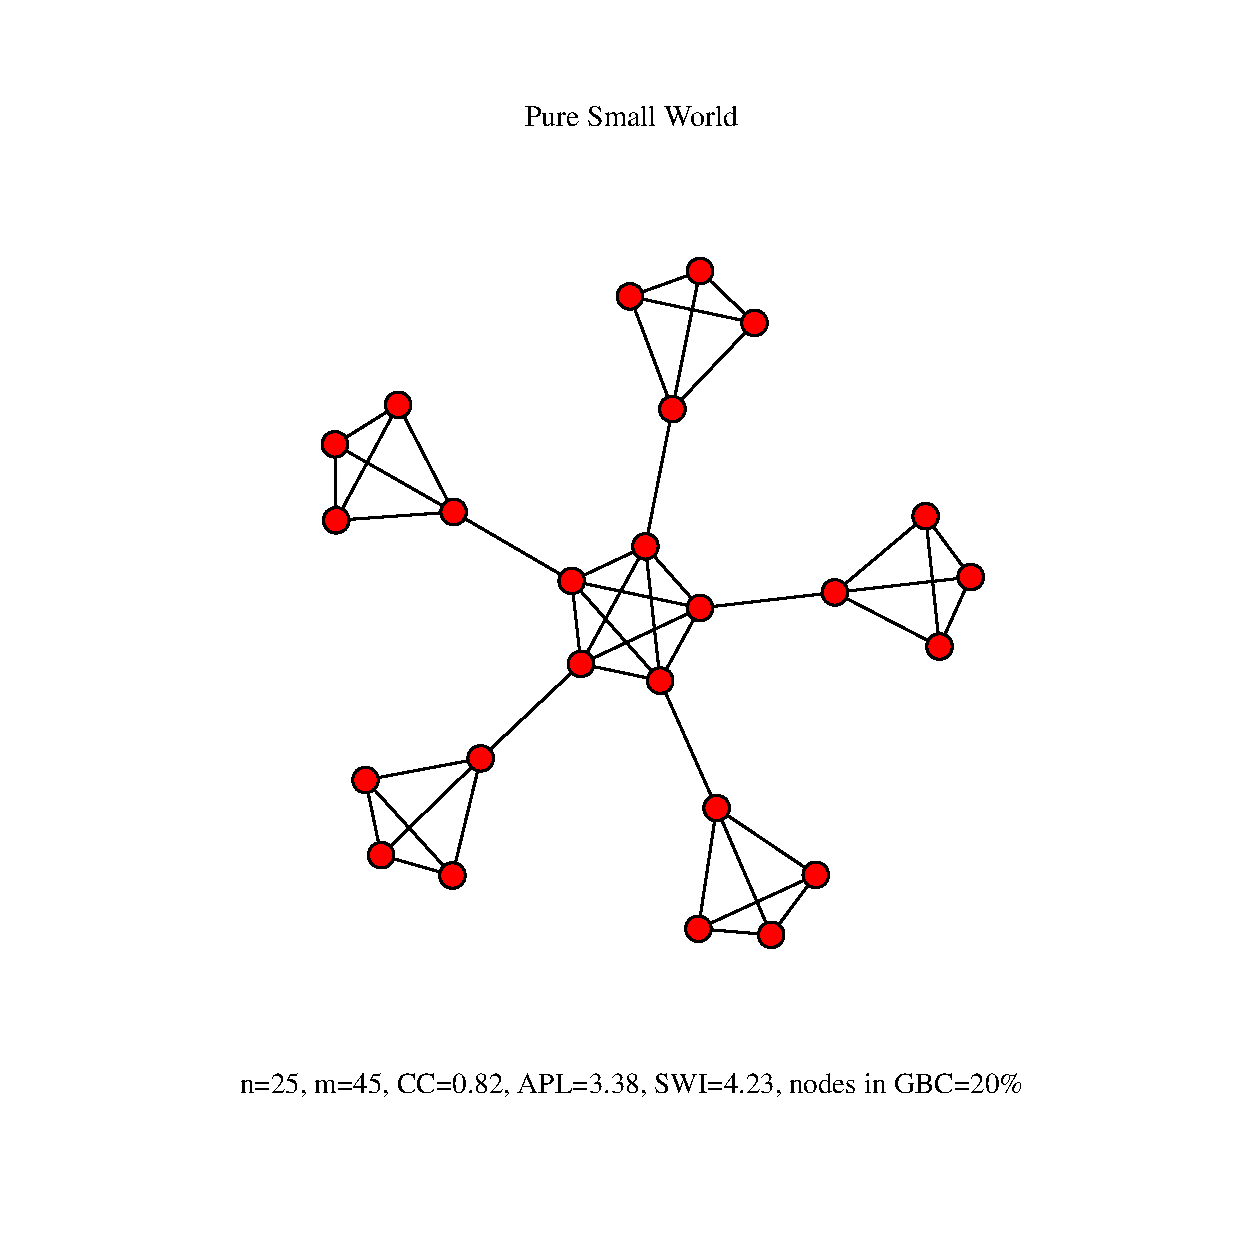
\includegraphics[scale=0.33]{figures/model_small_world_25}
}
\hspace{.05in}
\subfloat[Robustness pure structural cohesion]{
\label{fig:r_sc}
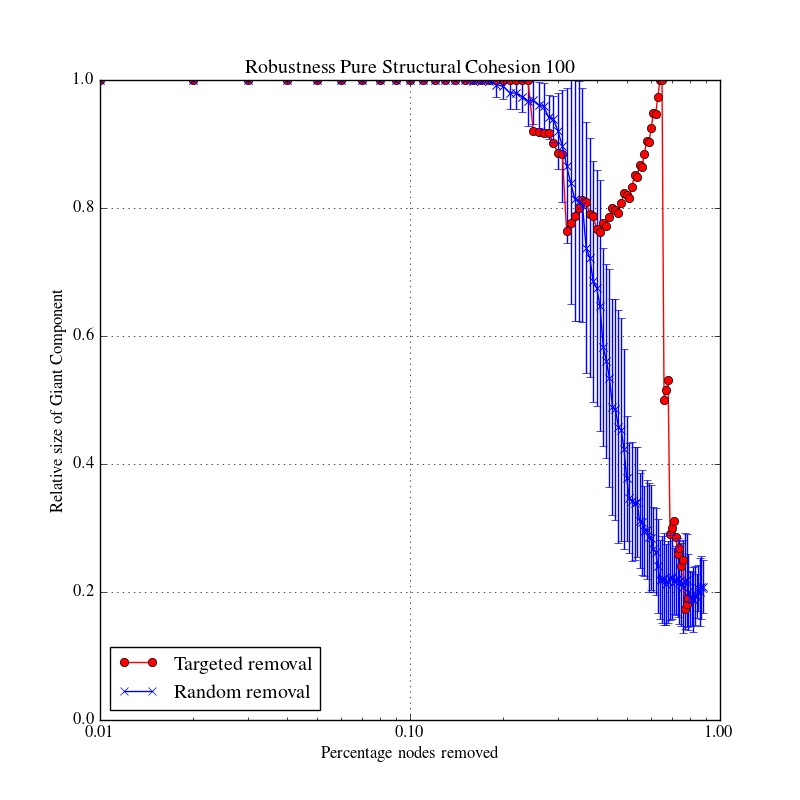
\includegraphics[scale=0.33]{figures/model_csen_log_Pure_Structural_Cohesion_100}
}
\hspace{.05in}
\subfloat[Robustness cohesive small world]{
\label{fig:r_csw}
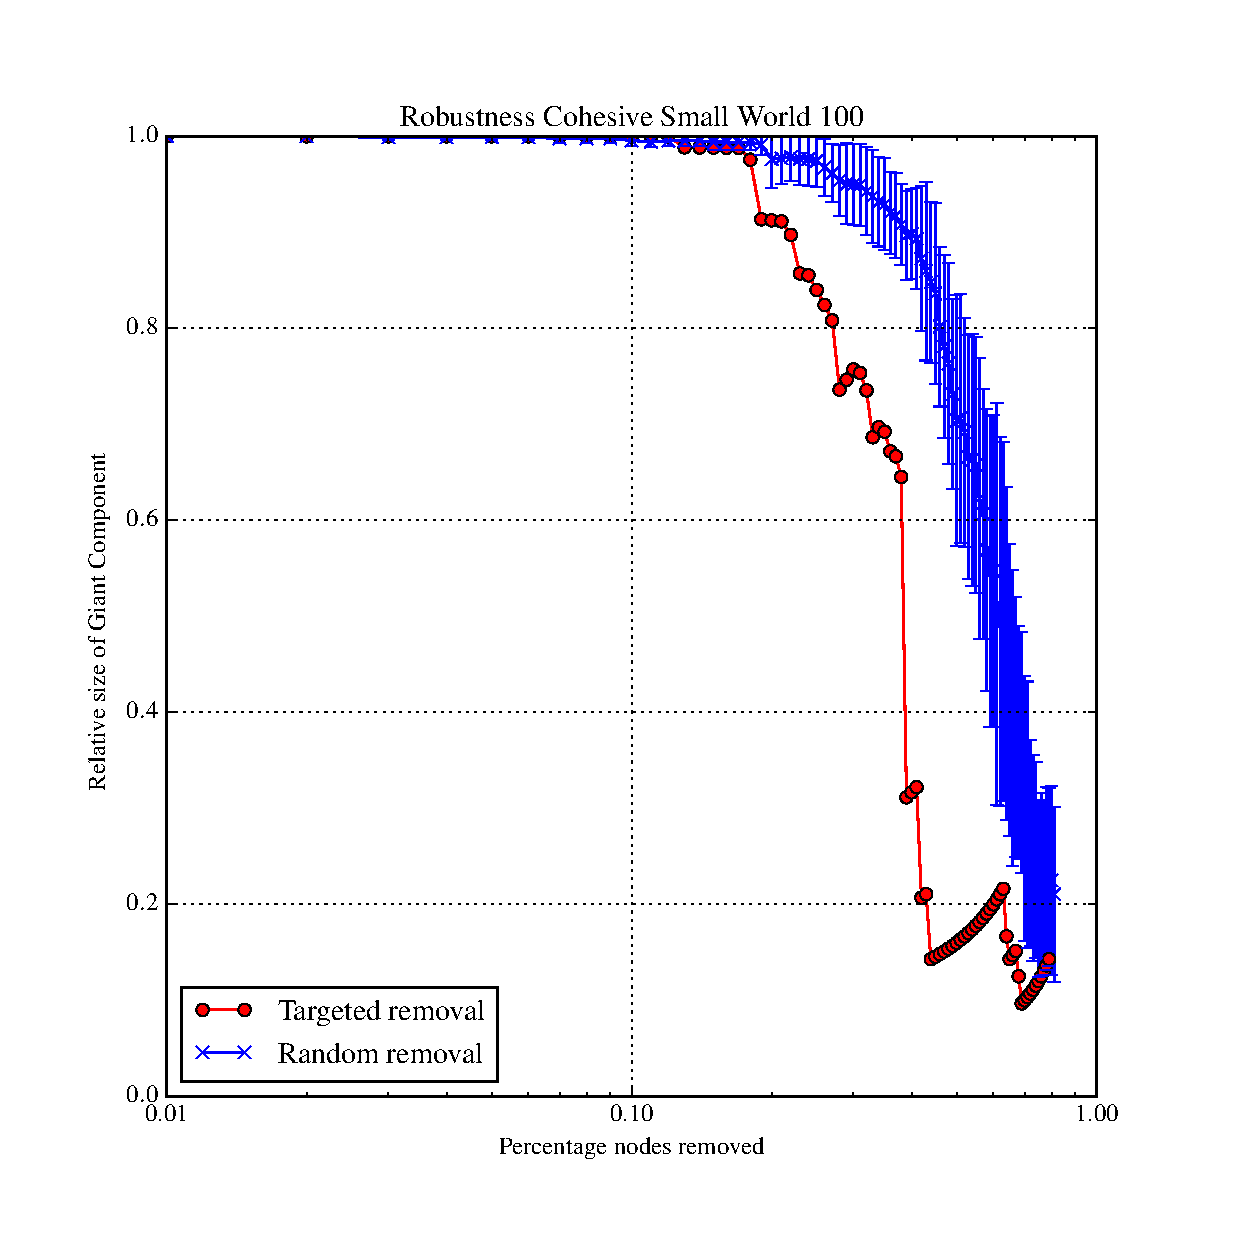
\includegraphics[scale=0.33]{figures/model_csen_log_Cohesive_Small_World_100}
}
\hspace{.05in}
\subfloat[Robustness pure small world]{
\label{fig:r_sw}
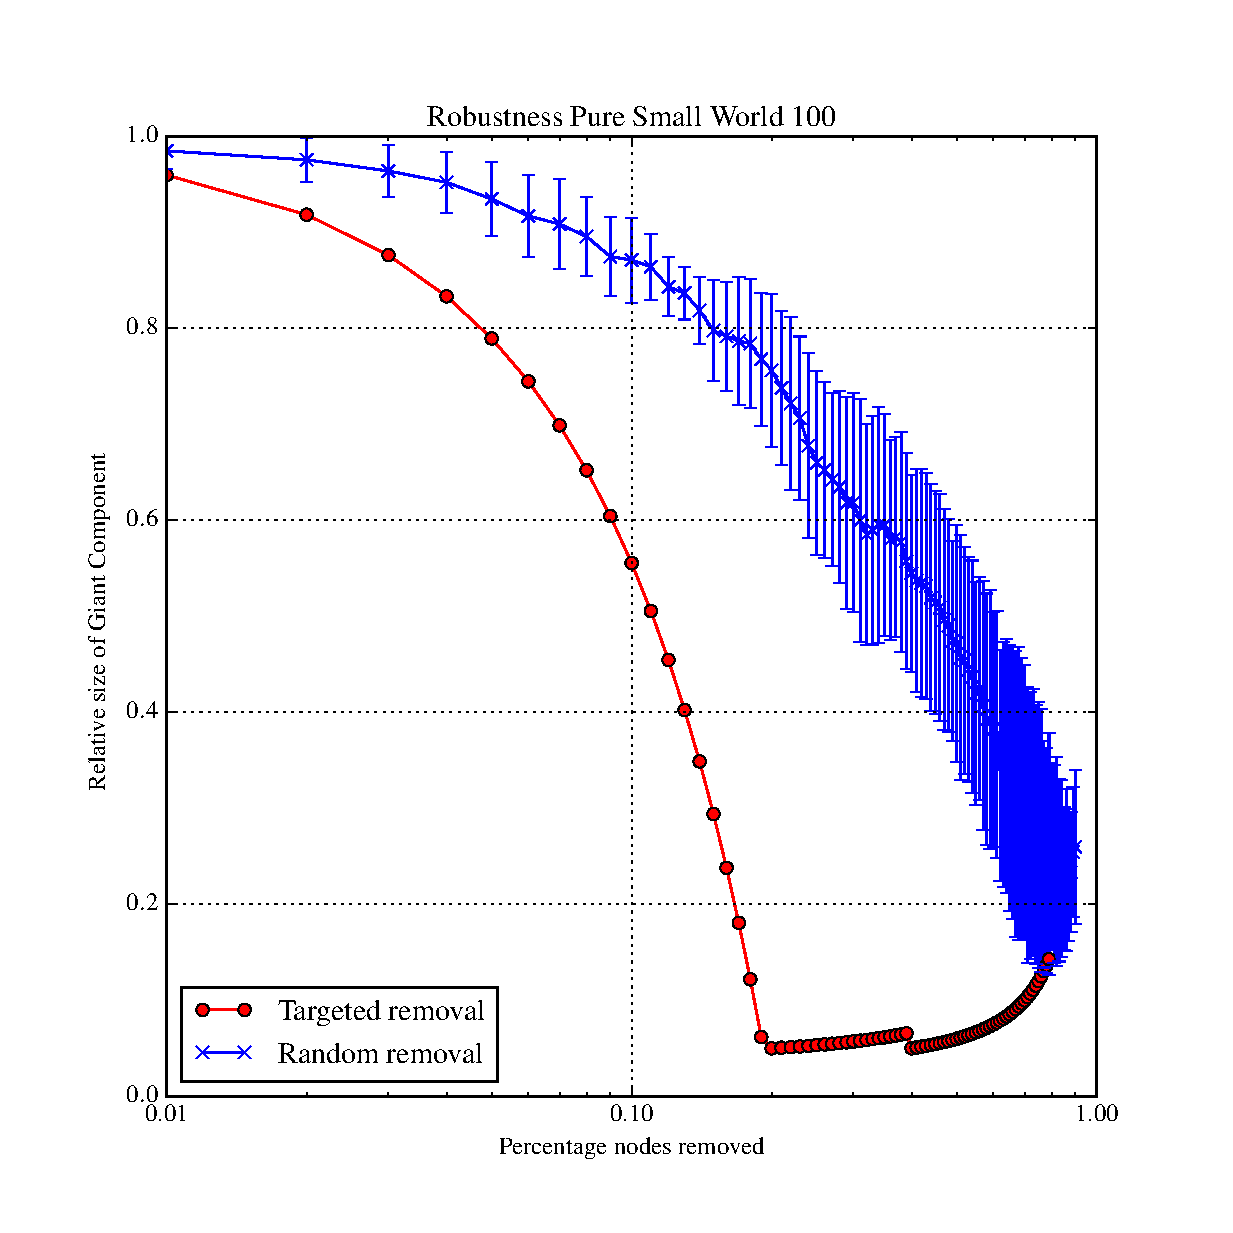
\includegraphics[scale=0.33]{figures/model_csen_log_Pure_Small_World_100}
}

\caption[Models of network structure and their robustness.]{Models of network structure and their robustness. The plots of the example networks (figures \ref{fig:sc_grid}, \ref{fig:csw} and \ref{fig:sw}) contain 25 nodes in order to facilitate the perception of their structure. The robustness plots (figures \ref{fig:r_sc}, \ref{fig:r_csw} and \ref{fig:r_sw}) are generated by toy networks of 100 nodes because the robustness pattern is clearer than in the 25 nodes examples. I also tested the robustness of all the models with 400 and 2500 nodes and the patterns are the same.}
\label{fig:models}
\end{figure}
\end{landscape}

